%
% File naaclhlt2012.tex
%
% Contact: nasmith@cs.cmu.edu

\documentclass[11pt,letterpaper]{article}
\usepackage{naaclhlt2012}
\usepackage{times}
\usepackage{latexsym}
\setlength\titlebox{2.5cm}    % Expanding the titlebox
\usepackage{graphicx}

\newcommand{\mnote}[1]{\marginpar{\raggedleft\footnotesize\itshape#1}} 


\title{Domain Adaptation for Paraphrasing}

%\author{Tsz Ping Chan \\
%  \small Johns Hopkins University\\
%  \small Baltimore, MD 21218, USA \\
%  {\tt \footnotesize tsz@jhu.edu} \\\And
%  \small Chris Callison-Burch \\
%  \small Johns Hopkins University\\
%  \small Baltimore, MD 21218, USA \\
%  {\tt \footnotesize ccb@cs.jhu.edu} \\\And
%  Benjamin Van Durme\\
%  \small HLTCOE\\
%  \small Johns Hopkins University\\
%  \small Baltimore, MD 21218, USA \\  
%  {\tt \footnotesize vandurme@cs.jhu.edu} \\}

\date{}

\begin{document}
\maketitle
\begin{abstract}
Paraphrases are typically tailored towards general domain of texts. Paraphrase extraction for a target domain can lead to poor phrase coverage and low quality paraphrases due to the lack of in-domain data. In this paper, we %adopt the data selection method introduced by  \newcite{moore-lewis:2010:Short}, which is based on the difference in cross entropy, to subsample data relevant to an in-domain text from a large general domain corpus. 
developed a framework for domain-specific paraphrasing, which applies cross-entropy difference subsampling introduced by \newcite{moore-lewis:2010:Short} to a multilingual paraphrase acquisition scheme. 
We compare the paraphrase quality for %biology, sports and parliamentary 
multiple domains and empirically demonstrate that domain-biased paraphrases resulting from our method is substantially more relevant to and contains more coverage of its source domain. Experimental results also indicates an improvement in the substitution task with domain-adapted paraphrases.

\end{abstract}

\section{Introduction}
\label{sect:intro}

Paraphrasing is a method of re-expressing a phrase that preserves the original meaning, usually within a certain context. Data-driven paraphrase acquisition approaches can be grouped into several categories depending on the data used for training. Monolingual paraphrasing methods uses statistical characteristics extracted from monolingual resources, such as dependency path similarities or distributional co-occurrence information \cite{Lin01discoveryof,PascaDienes05}. Bilingual paraphrasing techniques extract paraphrase candidates by grouping English phrases that share common foreign translations in parallel corpora \cite{BannardCallisonBurch05}. Additional paraphrase extraction methods fall between the two extremes, such as utilizing multiple English translation of the same foreign text or drawing knowledge from statistical machine translation to monolingual resources \cite{Barzilay2001,PangEtAl03,QuirkDolanBrockett04}.

%% Ben ===
Existing work in paraphrase acquisition has focussed on the
open-domain setting.  This leads to results that are
subjectively intuitive, and sometimes useful in unconstrained
settings, but are potentially less useful when working in a specific
domain such as chemistry, literature or art. 
%For example, the task of text-to-text re-writing has a variety of potential
%applications to an education setting.  In many such cases, the
%material to be processed will be specific to a field; chemistry,
%literature, art, etc. 
Consider the biology domain: morphological variants of the word
\emph{divide} may often be synonymous with variants of
\emph{multiply}, such as in: \emph{cell division}, and \emph{cell
  multiplication}.  This ambiguity is unlikely to hold in the
mathematics domain, or even in general text.  
%Table \ref{divide-example} gives more example of how 
%the paraphrases of {\it divide} are significantly different across two 
%domains.
Simply increasing the training corpus size for domain-specific paraphrasing is infeasible, since data-driven paraphrase acquisition techniques require large amount of training data and prepackaged in-domain training data is hard to come by in most domains. %Due to the fact the lack of definite metric of measuring paraphrase quality, machine learning techniques for training a classifier to, for example, assign a "domain score" would be difficult to apply in this problem 

We construct a framework of domain adaptation for paraphrasing by first intelligently subsampling a domain-specific parallel corpus from a much larger general domain of text using a metric developed by \newcite{moore-lewis:2010:Short}. We then %exploit two main paraphrase techniques by applying
apply monolingual similarity scores to the paraphrase candidates generated based on the domain-specific subsampled corpus using the pivot-based bilingual procedure. %For  defining the domain-of-interest with a biology textbook, we
We show that the domain-biased paraphrases generated by our method are more relevant to the %biology
target domain than without the domain-adapted subsampling. In addition, experimental results illustrate that domain adaptation positively impacts the substitution quality of paraphrases.



%@@ add content about BiP and MonoDS

%@@ emphasize reduction of computational resources required: memory/space for system(/paraphrase table) training, instead of interpolating of scores from domains or including the data in parameter estimation; uncouple learning from additional data from the process of system training with additional data. 

%In this paper, we suggest exploring domain adaptation for paraphrasing
%as an efficient method for tackling word sense disambiguation in the context of paraphrase acquisition.

%We might view this as a problem of \emph{word (phrase) sense ambiguity}: a given surface form
%may have different meanings, in different contexts.  
%could take a variety forms, , and word sense
%induction (WSI) for paraphrasing.

%% === Ben

\section{Related Work}
\label{sect:related_work}


\subsection{Domain Adaptation for SMT}
\label{sect:relatedWork_DA}
\newcite{daumeiii-kumar-saha:2010:DANLP} proposed a domain adaptation approach for SMT in a fully supervised setting. For an existing learning a function that maps vectors from an input space to a decision/output space, their approach expands each dimension in the input feature space (K + 1)-fold, where K is the number of domains. The training procedure which optimizes it�s performance on target (in-domain) data takes into account the additional information about the domain from which the data is collected. This paradigm trades additional domain information for increased computational burden due to the increase of feature space. Moreover, this adaptation procedure is implicitly restricted to certain structures of end-to-end tasks since it is incorporated directly into the machine translation task for both training and testing. These reasons makes such adaptation inapplicable for our paraphrasing framework.


%Frustratingly Easy Domain Adaptation, Hal Daume III, 2007
%		? ? the goal of our domain adaptation is to expand target domain data to 
%     train some *other* system/model; no explicit output space Y for the 
%     paradigm introduced by Hal
%         - domain adaptation for *classifier*
%	- NO subsampling
%	- no reduction of computation burden
%		- some parts of the pipeline for ppTable extraction requires batch computation, essential to reduce data volume while maintaining data quality
%	- increased feature space for classifier
%	- ourMethod: can intelligently select subset of "source domain" while
%		maintaining original structure of classifier feature space
%- a means to enhance feature space for a particular task
%	- ourWork: no end to end task, just subsampling to improve the quality of paraphrase for a particular domain 

%- training of the addition feature augmentation does not explicitly yield the degree of relevance of the additional text to the target domain; classifier features from the additional text are only considered jointly with the features from other domains to enhance the specific task at hand

\newcite{Schroeder07experimentsin} carried out experiments to compare end-to-end machine translations performance in terms of translation scores (BLEU) for a range of domain adaptation techniques applied to training data selection. Some of the techniques include in-domain language model, interpolating language model to bias towards specific domains, and simply combining training data. They showed that best BLEU scores are achieved with by adapting the training data to the domain of interest using language models. 
     
     
%@@  "A Generate and Rank Approach to Sentence Paraphrasing" by Malakasiotis and Androutsopoulos http://nlp.cs.aueb.gr/pubs/emnlp2011.pdf @@

%@@ Zhao's work @@

%@@ Interpolating paraphrase models traine \cite{Bellegarda04statisticallanguage}


% ===== 
%\paragraph{Domain Adaption for Paraphrasing}
\newcite{YarowskyACL95} introduced the notion of \emph{one sense per
discourse} to WSD, where a word or phrase in a given document, or
perhaps a collection of related documents, will tend to have just a
single sense.  This suggests that in order to extract paraphrases
that avoid the problems of WSD, we might simply restrict ourselves
to parallel corpora (when using bilingual pivot-based methods) that
fall in the domain of interest.
%
However, it is not obvious where one would naturally find large
collections of parallel data, precompiled according to specific
domains.  

We therefore propose to automatically induce \emph{domain-biased} parallel corpora, through extending the method proposed
by \newcite{moore-lewis:2010:Short} for building custom training corpora
for MT.  In the context of language model training, \newcite{moore-lewis:2010:Short} compared data selection methods such as in-domain cross-entropy scoring, similar to those used in \newcite{Schroeder07experimentsin}, Klakow's method \cite{Rajasekaran05selectingarticles} and cross-entropy difference scoring. They showed that difference in cross entropy results in the lowest perplexity in the test set of a specific target domain. The details of their model elaborated in Section \ref{sect:diffCE}.

In the first stage of our domain-bias paraphrasing framework, we begin with constructing an in-domain statistical language model with a monolingual collection of domain specific content.
A separate "general-domain" language model is then constructed for a
collection made up of uniformly at random sampled material from 
the English side of a large collection of mixed domain parallel text.
Each sentence in the remaining parallel corpus is scored based
on the difference in cross entropy (diffCE) from the language models.
Domain-biased subsampling retains sentences that satisfy certain
threshold on the diffCE. The subsampled parallel corpus is subsequently fed into a paraphrase extraction pipeline.

%The domain adaptation technique we examined selects documents based on the difference in cross entropy (CE) between an in-domain language model and a general/out-of-domain language model. Because this technique is monolingual, it enables a joint experiment of using this method to influence the monolingual distributional similarity scores.  For instance, instead of uniformly weighting the contexts for each instance of a phrase, we can weight these based on the difference in CE, or based on how much each context appears to be similar to the domain of interest. 

%  ======

%\subsection{Paraphrase Extraction}
%\label{sect:}


\subsection{Paraphrase Acquisition from Bitexts}
\label{sect:BiP}

%% ====== extracted from GEMS
 \newcite{BannardCallisonBurch05} proposed identifying paraphrases by pivoting through phrases in a bilingual parallel corpora. 
Figure~\ref{paraphrase-illustration} illustrates their paraphrase extraction process. The \emph{target} phrase, e.g. {\it thrown into jail}, is found in a German-English parallel corpus.  The corresponding foreign phrase ({\it festgenommen}) is identified using word alignment and phrase extraction techniques from phrase-based statistical machine translation \cite{KoehnEtAl03}.  Other occurrences of the foreign phrase in the parallel corpus may align to a distinct English phrase, such as {\it jailed}.  
%Following \newcite{BannardCallisonBurch05}, we treated any English phrases that share a common foreign phrase as potential paraphrases of each other.
%
As the original phrase occurs several times and aligns with many different foreign phrases, each of these may align to a variety of other English paraphrases.  Thus, {\it thrown into jail} not only paraphrases as {\it jailed}, but also as {\it arrested}, {\it detained}, {\it imprisoned}, {\it incarcerated}, {\it locked up}, and so on.
%{\it taken into custody}, and {\it thrown into prison} and others like {\it be thrown in prison}, {\it been thrown into jail}, {\it being arrested}, {\it in jail}, {\it in prison}, {\it put in prison for}, {\it were thrown into jail}, and {\it who are held in detention}. 
Bad paraphrases, such as
 {\it maltreated}, {\it thrown}, {\it cases}, {\it custody}, {\it arrest}, and {\it protection}, may also arise due to poor word alignment quality and other factors.

\newcite{BannardCallisonBurch05} defined a paraphrase probability to rank these paraphrase candidates,  as follows:
\begin{eqnarray} 
 \hat{e_2}	& = & \arg \max_{e_2 \neq e_1} p(e_2 | e_1)\label{paraphrase-prob}  \\
  p(e_2|e_1) &=& \sum_f p(e_2,f|e_1)\\
                  &=& \sum_f p(e_2|f,e_1) p(f|e_1) \\
                  &\approx& \sum_f p(e_2|f) p(f|e_1)
\label{paraphrase_prob_eqn}
\end{eqnarray}
where ${p(e_2|e_1)}$ is the paraphrase probability, and ${p(e|f)}$ and ${p(f|e)}$ are translation probabilities from a statistical translation model.  


\begin{figure}
\begin{center}
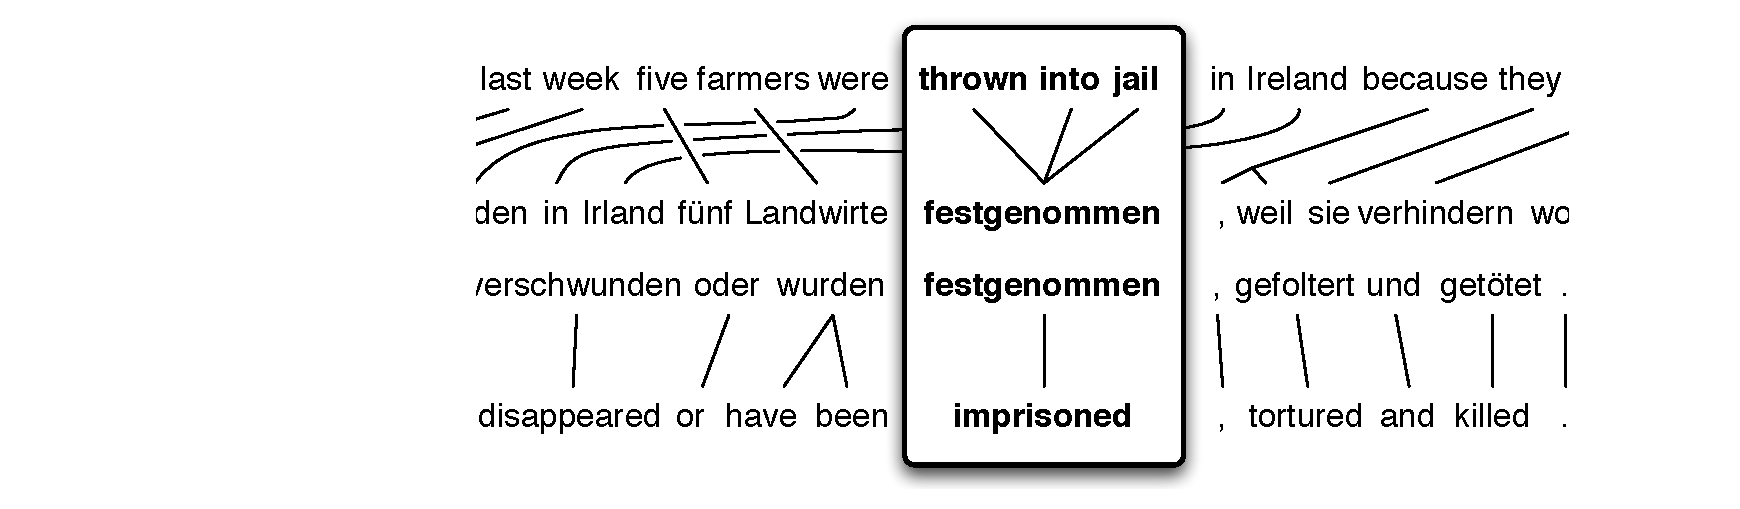
\includegraphics[width=\linewidth]{pivot-2}
\end{center}
%\vspace{-.35cm}
\caption{\small Using a bilingual parallel corpus to extract paraphrases.\vspace{-.12cm}}
\label{paraphrase-illustration}
\end{figure}

Anecdotally, this paraphrase probability sometimes seems unable to discriminate between good and bad paraphrases, so some researchers disregard it and treat the extracted paraphrases as an unsorted set \cite{Snover2010}.  \newcite{CallisonBurch08} attempts to improve the ranking by limiting paraphrases to be the same syntactic type.  

We attempt to rerank the paraphrases using other information. This is similar to the efforts of \newcite{ZhaoEtAlACL08}, who made use of multiple resources %, namely the thesaurus, monolingual parallel corpus, monolingual comparable corpus, bilingual phrase table, dictionary definitions, clusters of similar user queries, and self paraphrase 
to derive feature functions and extract paraphrase tables. The paraphrase that maximizes a log-linear combination of various feature functions is then selected as the optimal paraphrase. Feature weights in the model are optimized by minimizing a {\it phrase substitution error rate}, a measure proposed by the authors, on a development set.
% ===========

\subsection{Monolingual Distributional Similarity}
\label{sect:MonoDS}

%% ====== extracted from GEMS
Prior work has explored the acquisition of paraphrases using distributional
similarity computed from monolingual resources, such as in the DIRT results of
\newcite{Lin01discoveryof}. In these models, phrases are judged to be similar
based on the cosine distance of their associated context vectors. In some cases,
such as by Lin and Pantel, or the seminal work of \newcite{ChurchHanks91},
distributional context is defined using frequencies of words appearing in
various syntactic relations with other lexical items. For example, the nouns
\emph{apple} and \emph{orange} are contextually similar partly because they both
often appear as the object of the verb \emph{eat}. While syntactic contexts
provide strong evidence of distributional preferences, it is computationally
expensive to parse very large corpora, so it is also common to represent context
vectors with simpler representations like adjacent words and n-grams
\cite{LapataKellerSaLP05,BhagatRavichandran08,LinEtAlLREC10,VanDurmeLallACL10}. In
these models, \emph{apple} and \emph{orange} might be judged similar because
both tend to be one word to the right of \emph{some}, and one to the left of
\emph{juice}.

Here we calculate distributional similarity using a web-scale n-gram corpus
\cite{GoogleNgrams,LinEtAlLREC10}. Given both the size of the collection, and
that the n-grams are sub-sentential (the n-grams are no longer than 5 tokens by
design), it was not feasible to parse, which led to the use of n-gram contexts.  Here we use adjacent unigrams.
For each phrase $x$ we wished to paraphrase, we extracted the context vector of
$x$ from the n-gram collection as such: every (n-gram, frequency) pair of the
form: ($a x$, $f$), or ($x b$, $f$), gave rise to the (feature, value) pair:
($w_{i-1}$=$a, f$), or ($w_{i+1}$=$b, f$), respectively. In order to scale to this
size of a collection, we relied on Locality Sensitive Hashing (LSH), as was done
previously by \newcite{ravichandranACL05} and \newcite{BhagatRavichandran08}. To
avoid computing feature vectors explicitly, which can be a memory intensive
bottleneck, we employed the online LSH variant described by
\newcite{VanDurmeLallACL10}.

This variant, based on the earlier work of \newcite{IndykSTOC98} and
\newcite{Charikar02}, approximates the cosine similarity between two feature
vectors based on the Hamming distance in a reduced bit-wise representation. In
brief, for the feature vectors $\vec{u}$, $\vec{v}$, each of dimension $d$, then
the cosine similarity is defined as: $\frac{\vec{u} \cdot
  \vec{v}}{|\vec{u}||\vec{v}|}$. If we \emph{project} $\vec{u}$ and $\vec{v}$
through a $d$ by $b$ random matrix populated with draws from $N(0,1)$, then we
convert our feature vectors to \emph{bit signatures} of length $b$, by setting
each bit of the signature conditioned on whether or not the respective projected
value is greater than or equal to 0. Given the bit signatures $h(\vec{u})$ and
$h(\vec{v})$, we approximate cosine with the formula:
$\cos(\frac{D(h(\vec{u}),h(\vec{v}))}{b}\pi)$, where $D()$ is Hamming distance.
% ==========


\section{Domain Adaptation}
\label{sect:DA}

\subsection{Data Selection based on Difference in Cross Entropy}
\label{sect:diffCE}

As briefly introduced in Section \ref{sect:related_work}, \newcite{moore-lewis:2010:Short} proposed an approach for subsampling of a non-domain specific corpus based on difference in cross entropy with respect to in-domain and general-domain language models. The goal of their work was to exploit a large corpus efficiently in terms of computational resources to enhance for specific machine translation tasks. In their method, a substantially larger general-domain corpus is randomly subsampled to match the size of the much smaller in-domain text. Separate language models are trained with the in-domain text and smaller general-domain corpora, with the assumption that enough data was used to train an effective language model. The cross entropy of individual sentences in the remaining general-domain corpus are calculated according to the language models. 

Since a smaller value in cross entropy implies the closer resemblance of a sentence to the domain of the language model, the difference in cross entropy can serve as metric for selecting a subset of the non-domain-specific corpus that matches more with the in-domain data than the out-of-domain data. Moore and Lewis showed that, across a range of subsampled data sizes, their subsampling method produced much smaller perplexity for in-domain test data as compared to methods such as Klakow's method, in-domain cross-entropy scoring and random selection.

%%%
%In our framework, we used the content of biology textbook to construct an in-domain statistical language model with a monolingual collection of domain specific content, such as the pages of a biology textbook.
%A separate "general-domain" language model is then constructed for a
%collection made up of uniformly at random sampled material from 
%the English side of a large collection of mixed domain parallel text.
%Each sentence in the remaining parallel corpus is scored based
%on the difference in cross entropy (diffCE) from the language models.
%Domain-biased subsampling retains sentences that satisfy certain
%threshold on the diffCE. The subsampled parallel corpus is subsequently fed into a paraphrase extraction pipeline.

In our work, we utilize this data selection method as a means to bias the relevance of our paraphrases to a domain of interest.
% Although learning (larger size, better learning, but proved not the case here?)
%% ==== from DomainAdaptationDescription.doc
The overall domain adaptation procedure is illustrated in Figure 1. After the in-domain and out-of-domain language models are trained with the respective training data, they are used to calculate the cross entropy for the sentences in rest of the out-of-domain text. For a particular sentence {\em s}, the difference in cross entropy, defined as ${\Delta}$H({\em s}) = H$_{IN}$({\em s}) - H$_{OUT}$({\em s}), is used to categorize it into one of N bins, which all contain roughly the same number of sentences and are specified by the range of cross entropy difference values. The larger a ${\Delta}$H({\em s}) value is, the closer to the in-domain text this sentence {\em s} is.

The corresponding translation of the sentences in the top bins are retrieved from the out-of-domain parallel corpus and result in a domain-adapted parallel corpus. This subsampled text then undergoes the standard bilingual pivoting framework for extracting a collection of phrases and the associated domain-adapted paraphrases. 

There is a trade-off between the amount of data for paraphrase extraction and the relevance of the paraphrases to the in-domain text. A larger number of top bins used for constructing a paraphrase table would lead to more coverage and confidence of the paraphrases, but the paraphrases would also be less applicable to the specific domain of interest.
% =====

%%%
%@@ add introducing 2 models
%
%...
%Next, for each document in the parallel corpus outside the
%training material, a score is assigned based on the ``closeness'' of
%the document to the in-domain language model, as compared to the
%general-domain.  This score will then be used either in weighting the
%resultant rule extraction probabilities, or in a coarser-grained
%approach, by simply creating a small parallel collection by
%filtering those documents deemed too ``far'' from the target domain.
%




% Pipeline diagram
\begin{figure*}
\begin{center}
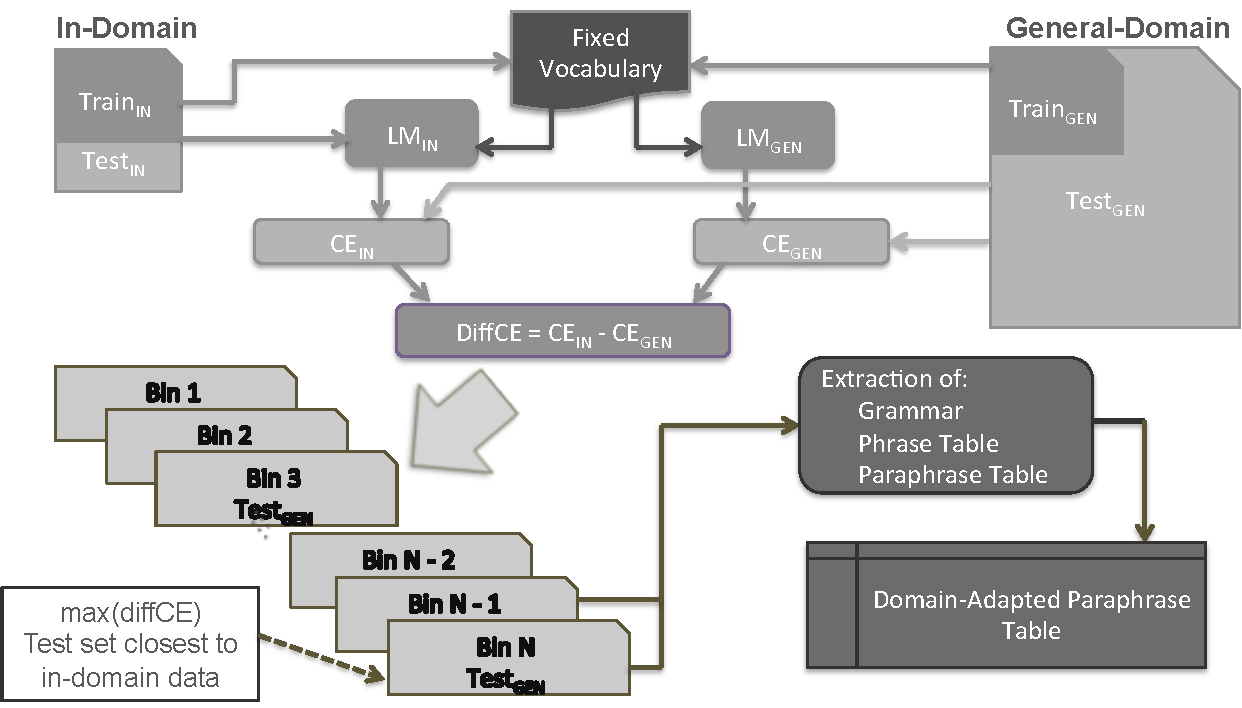
\includegraphics[width=.8\linewidth]{DomainAdaptationDiagram_BnW} %[width=\linewidth]
\end{center}
%\vspace{-.35cm}
\caption{\small Diagram of the domain adaptation procedure based on difference in entropy. LM, CE, diffCE stand for language model, cross entropy, and difference in cross entropy, respectively. Bins of out-of-domain test data are ordered based on their diffCE values, which is proportional to the "closeness" of each individual sentences to the targeted domain. N, denoting the number of bins, is 8 in our experiment.}
\label{pipeline_diagram}
\end{figure*}


\subsection{Domain Adaptation for Paraphrasing}
\label{sect:DA_pphrase}

Each stage in our paraphrase framework depends on different data statistics from its the training data, we therefore investigated the effectiveness of paraphrase biasing by applying domain adaptation independently to pivot-based paraphrase acquisition and monolingual reranking.

%{\bf Bilingual Pivoting}

For bilingual paraphrase acquisition, by biasing the domain of the parallel corpus from which grammar is extracted, the phrase table would potentially be dominated by content with more frequent uses in that specific domain. Hence, the resulting coverage and probability of paraphrases after bilingual pivoting are both expected to be closer to the domain of interest. 

%{\bf Monolingual Distributional Similarity}

The similarity score based on monolingual distributional similarity (MonoDS) was originally proposed to be computed using the Google ngram corpus \cite{LinEtAlLREC10}, which comprises of statistics from general domain of resources on the internet. While large amount of data might lead to a better vector space model for the MonoDS score, adapting a training corpus to the target domain can potentially enhance the relevance of the paraphrases reranking.

%{\bf Log-linear Model Training}

%difference in cross entropy as weight

\section{Experimental Setup}
\label{sect:exptSetup}

We have evaluated the effects of domain bias for various aspects of paraphrasing such as coverage, perplexity on test data, and empirical examples. The details of the experimental setup covered in the rest of this section are described with reference to the diagram in Figure \ref{pipeline_diagram}. 

\subsection{Data and Language Models}
\label{sect:data_LMs}

%@@ data: in-domain, out-domain
%% === from DomainAdaptationDescription.doc
%% In-domain corpus and fixed vocabulary for LM training

{\em Language Models Training Data} The majority of our evaluation is based on a target domain defined by biology-related context. We built our target domain language model by combining a biology textbook and the GENIA database \cite{jdkim:2003}, which are of similar sizes. The GENIA database is a collection of 1.999 biomedical publication abstracts, whereas the biology textbook is text material intended for generic introductory courses in biology.

Another domain of text used for domain biasing is parliamentary, which was extracted from proceedings of the European parliament with a total of about 97 million words in the English-translation text. For the results from different language models to be comparable, the language models training data must be similar in sizes. 
%Out of the (size) tokens in this collection, disjoint sets in the sizes of 

%% === 
GigaFrEn, a French-English parallel corpus verging on 1 billion words \cite{callisonburch-EtAl:2009:WMT} was used as the general corpus from which the domain-specific corpus is built. It was constructed by conducting a large-scale web crawl targeting bilingual web sites. It captures a wide variety of topics\footnote{These sites came from a variety of sources including the Canadian government, the European Union, the United Nations, Amnesty International, the World Health Organization, and other international organizations. The crawl yielded on the order of 40 million files, consisting of more than 1TB of data. It represents the largest and most diverse parallel corpus available for research purposes.}, and is therefore perfectly suited for domain-adaptation studies for bilingually derived paraphrases.

The non-domain-specific data consists of the Giga-French-English  and the Europarl French-English corpora, which sum up to roughly 0.6 billion words on the English side. The language models for cross entropy calculations were trained separately on data set of similar sizes to allow for comparable results. 
 %% ===
 
{\em Language Model Vocabulary} A list of fixed vocabulary extracted from the unigrams in the in-domain training data and the textbook index, were used to train both of the language models. Preprocessing on the training data was performed in order to eliminate lines with non-sentence like structure or with too many special or repeated characters. Unigrams from the biology textbook was required to have repeated occurrences in order to be included in the vocabulary list.


{\em Preprocessing}@@ tokenization, normalization, cleaning, all preprocessing (see fileInfo.txt notes and refer to first paragraphs of Moore's section 3)

@@ srilm model params
@@ thresholding in BiP and MonoDS scores
@@ averaging in analysis: mean sent, median turker
@@ emphasize what's used as "in-domain test set" and will be used repeatedly for quantitative evaluation in subsequent sections


\subsection{Language Model Training for In-Domain Text}
\label{sect:LM_PPL}



\subsection{Paraphrase Extraction}
\label{sect:method_pphrase}
@@ take content from GEMS Sect 3.3?
The parallel corpus    The bilingual pivoting 


@@ examples


%\begin{table}
%\begin{center}
%\begin{tabular}{ll}
%\hline\hline 
%\multicolumn{2}{c}{\bf \footnotesize \emph{divide}}\\ \hline
%\footnotesize {\bf parliamentary } & \footnotesize{\bf biology }\\ \hline
%{\scriptsize \emph{gap}}	&	{\scriptsize \emph{divided	}}	\\
%{\scriptsize \emph{division}}	&	{\scriptsize \emph{division}}	\\
%{\scriptsize \emph{split}}	&	{\scriptsize \emph{dividing}}	\\
%{\scriptsize \emph{divided}}	&	{\scriptsize \emph{divides}}	\\
%{\scriptsize \emph{gulf}}	&	{\scriptsize \emph{break}}	\\
%{\scriptsize \emph{dividing}}	&	{\scriptsize \emph{split}}	\\
%{\scriptsize \emph{share}}	&	{\scriptsize \emph{dispense}}	\\
%{\scriptsize \emph{divide up}}	&	{\scriptsize \emph{multiply}}	\\
%{\scriptsize \emph{divisions}}	&	{\scriptsize \emph{cleave}}	\\
%{\scriptsize \emph{separate}}	&	{\scriptsize \emph{fracture}}	\\
%{\scriptsize \emph{distinction}}	&	{\scriptsize \emph{separate}}	\\
%{\scriptsize \emph{rift}}	&	{\scriptsize \emph{mitotic division}}	\\
%{\scriptsize \emph{difference}}	&	{\scriptsize \emph{partition}}	\\
%\hline
%\end{tabular}
%\vspace{-.25cm}
%\end{center}
%\caption{Potential paraphrases of \emph{divide} drawn from two different domains.}
%\label{divide-example} 
%%\vspace{-.57in}
%\end{table}


%%%%%%% add below content to comparison paragraphs


@@ 20111117b.rtf @@@
%%%%%%%%%%%%%%%%%%%%%%%%%%%%%%%%%


\section{Experimental Results}
\label{sect:expt_results}



\subsection{Subsampling Methods Comparison}
\label{sect:otherSubsampling}
% ================  Stats/setup for domain adaptation vs Random at various sample sizes ================ %
\begin{table}[t!]
\begin{center}
\begin{tabular}{ll|ll}%{|l|l|l|}
\hline\hline 
\multicolumn{2}{c|} {\bf \scriptsize DiffCE} & \multicolumn{2}{c} {\bf \scriptsize Random} \\
\hline
{\bf \footnotesize Line count}  & {\bf \footnotesize Token count} &{\bf \footnotesize Line count}  & {\bf \footnotesize Token count}\\
\hline
%\bf \footnotesize BiP & \bf \footnotesize SyntBiP & \bf \footnotesize BiP-MonoDS \\ \hline
{\scriptsize 1,271,750} & {\scriptsize 27,831,706} & {\scriptsize 1,270,000} & {\scriptsize 27,852,488} \\
{\scriptsize 2,543,466} & {\scriptsize 56,384,338} & {\scriptsize 2,540,000} & {\scriptsize 55,733,642}  \\
{\scriptsize 5,086,899} & {\scriptsize 119,776,920} & {\scriptsize 5,080,000} & {\scriptsize 111,478,225}  \\
{\scriptsize 10,173,762} & {\scriptsize 263,492,323} & {\scriptsize 10,160,000} & {\scriptsize 222,917,055}  \\
\hline
\end{tabular}
\end{center}
%\vspace{-.25cm}
\caption{Statistics of corpora used for domain adaptation} 
\label{tbl_steppedSizeStats}
\end{table}

Although domain-biased subsampling is expected to outperform random sampling, the common notion that "more data beats better algorithms" implies that the effect of domain-bias can potentially be masked by the size of a randomly subsampled corpus. To investigate the gain of applying domain adaptation to paraphrasing, corpora at various sizes are subsampled with each method and used for language model training independently. The line and token counts of each pair of corpora at different sizes are listed in Table \ref{tbl_steppedSizeStats}.


% ================  DiffCE vs JOSHUA ================ %
\begin{table}[t!]
\begin{center}
\begin{tabular}{l|c|c}%{|l|l|l|}
\hline\hline 
 & {\bf \scriptsize Line/Token count} & {\bf \scriptsize PPL$_{InDomain}$} \\
 \hline
{\bf \scriptsize DiffCE} & {\scriptsize 573,659 / 12,779,577} & {\scriptsize 319.2}\\
 {\bf \scriptsize Subsampling$_{Joshua}$} & {\scriptsize 573,659 / 10,667,535} & {\scriptsize 604.4}\\
\hline
\end{tabular}
\end{center}
%\vspace{-.25cm}
\caption{Statistics of corpora used for domain adaptation method comparison and the respective in domain {\em test} data perplexities (PPL$_{InDomain}$)} 
\label{tbl_subsampStats}
\end{table}

Due to computational constraints, research in MT typically employs simple subsampling methods in order to reduce the amount of data for actual processing. For example, a standard subsampling method based on n-gram overlap with a reference text for sentence selection is provided by Joshua \cite{Joshua-Decoder}, an open source decoder for statistical MT. In order to compare this subsampling method with that based on difference in cross entropy, the corpus of similar size to the Joshua subsampling was extracted based on diffCE. Table \ref{tbl_subsampStats} tabulates the corpora sizes and the perplexity for in-domain text data. The smaller perplexity produced by diffCE-based method validates cross entropy from two contrasting domains is more informative than basic n-gram overlap methods. This result also implies that, if computational resources is a constraint, the diffCE-based method would likely to deliver better performance for the same size of subsampling.


% ====================================%

	





% ================  COVERAGE ================ %
\begin{table}[t]
\begin{center}
\begin{tabular}{l|cccc|c}%{|l|l|l|}
\hline\hline 
&\multicolumn{4}{c|} {\bf \scriptsize N-gram} &\\
\hline
{\bf \footnotesize Corpus} & {\bf \footnotesize 1}& {\bf \footnotesize 2}& {\bf \footnotesize 3}& {\bf \footnotesize 4}& {\bf \footnotesize Total} \\
\hline
{\scriptsize Europarl} & {\scriptsize 11,536} & {\scriptsize 55,373} & {\scriptsize 42,540} & {\scriptsize 13,851}& {\scriptsize 123,300} \\
{\scriptsize Top} & {\scriptsize 16,771} & {\scriptsize 91,697} & {\scriptsize 67,737} & {\scriptsize 18,292} & {\scriptsize 194,497} \\
{\scriptsize Bottom} & {\scriptsize 9,022} & {\scriptsize 25,835} & {\scriptsize 11,575} & {\scriptsize 2,008}& {\scriptsize 48,440} \\
{\scriptsize Random}  & {\scriptsize 14,606} & {\scriptsize 66,656} & {\scriptsize 45,207} & {\scriptsize 11,616} & {\scriptsize 138,085} \\
\hline
{\scriptsize Textbook} & {\scriptsize 21,422} & {\scriptsize 212,408} & {\scriptsize 433,425} & {\scriptsize 512,515} & {\scriptsize 1,179,770} \\
\hline
\end{tabular}
\end{center}
\caption{Number of unique N grams in biology textbook that appear in the paraphrase tables generated with different subsampling methods, where {\em Top} and {\em Bottom} refer to the domain adapted domains closest and furthest from the domain of interest, respectively } 
\label{tbl_ppTableCoverage}
\end{table}
% source: ~tsz/vulcan/ppTableCoverageStats

Table \ref{tbl_ppTableCoverage} reports the overlap between the unique phrases of up to 4-gram from the biology textbook and each of the paraphrase tables generated from different subsampled corpora. Although all of the paraphrase tables were constructed with corpora of very similar sizes, the domain-biased paraphrase table, labeled as {\em Top}, contains the most number of phrases in the biology textbook across all 4 n-gram lengths. This highlights that intelligent selection of corpus for bilingual pivoting facilitates an increase of the paraphrase coverage for a task of interest.



% ================= Domain adaptation vs Random at various sample sizes ================== %
%
%\begin{table}[t!]
%\begin{center}
%\begin{tabular}{c|cc}%{|l|l|l|}
%\hline\hline 
%{\bf \footnotesize Size (Token)} & {\bf \footnotesize DiffCE} & {\bf \footnotesize Random} \\
%\hline
%%\bf \footnotesize BiP & \bf \footnotesize SyntBiP & \bf \footnotesize BiP-MonoDS \\ \hline
%{\scriptsize $\sim$28M} & {\scriptsize 329.5} & {\scriptsize 954.4} \\
%{\scriptsize $\sim$56M} & {\scriptsize 359.9} &{\scriptsize 856.9} \\
%{\scriptsize $\sim$111M}& {\scriptsize 424.7}& {\scriptsize 775.4} \\
%{\scriptsize $\sim$230M} & {\scriptsize 531.4} & {\scriptsize 699.4}\\
%\hline
%\end{tabular}
%\end{center}
%%\vspace{-.25cm}
%\caption{In-domain test data perplexity according to language models trained based on difference in entropy (DiffCE) and random sampling (random) as a function of sample size.} 
%\label{tbl_steppedSizePPL}
%\end{table}

\begin{figure}
\begin{center}
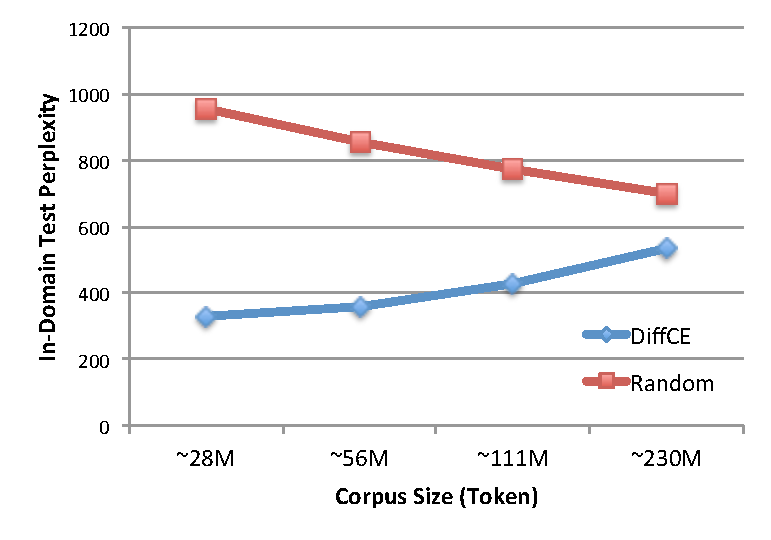
\includegraphics[width=1\linewidth]{stepSizeCmp} %[width=\linewidth]
\end{center}
\vspace{-.35cm}
\caption{\small In-domain test data perplexity according to language models trained based on difference in entropy (DiffCE) and random sampling (random) as a function of sample size.}
\label{stepSizeCmp}
\end{figure}


Domain adapting and random subsampling are compared in Figure \ref{stepSizeCmp} at various sizes as listed previously in Table \ref{tbl_steppedSizeStats}. The domain specific subsampling results in less perplexity than random selection throughout the two curves, which indicates that, at each of the increasing corpus sizes, the language model trained on the data subsampled with difference in cross entropy remains better at prediction than the baseline of random sampling. This plot is comparable to the empirical result obtained in \newcite{moore-lewis:2010:Short}, which suggested that diffCE is more effective in terms of test set perplexity as training set size decreases.

The reason for the perplexity curves to merge as corpus size increases is obvious: the domain-specific corpus grows by including sentences less related to the biology domain. At a size of about 230M tokens, which is about half the size of the original giga-French-English corpus, the two subsampling methods are expected to have large amount of overlap, hence resulting similar perplexity values. Such convergence of performance in both subsampling methods as the corpus size increases should not be a concern because under the scenario of interest,  intelligent subsampling would constitute an advantage when computational speed or storage is a limitation.


% ======================================== %
	
	

\subsection{Paraphrase Examples}
\label{sect:example_pphrases}

@@ Tables of examples
@@'host'
@@'channel'
@@'dynamic'
@@'water' or 'sodium hydroxide' or 'cholesterol'
@@'activation'
@@'peripheral'
@@get content from %20111110_LM_adapt_afterExtraction_examples.xlsx AND thresholded paraphrase tables

%\begin{table}
%\begin{center}
%\begin{tabular}{ll}
%\hline\hline 
%\multicolumn{2}{c}{\bf \footnotesize \emph{divide}}\\ \hline
%\footnotesize {\bf parliamentary } & \footnotesize{\bf biology }\\ \hline
%{\scriptsize \emph{gap}}	&	{\scriptsize \emph{divided	}}	\\
%{\scriptsize \emph{division}}	&	{\scriptsize \emph{division}}	\\
%{\scriptsize \emph{split}}	&	{\scriptsize \emph{dividing}}	\\
%{\scriptsize \emph{divided}}	&	{\scriptsize \emph{divides}}	\\
%{\scriptsize \emph{gulf}}	&	{\scriptsize \emph{break}}	\\
%{\scriptsize \emph{dividing}}	&	{\scriptsize \emph{split}}	\\
%{\scriptsize \emph{share}}	&	{\scriptsize \emph{dispense}}	\\
%{\scriptsize \emph{divide up}}	&	{\scriptsize \emph{multiply}}	\\
%{\scriptsize \emph{divisions}}	&	{\scriptsize \emph{cleave}}	\\
%{\scriptsize \emph{separate}}	&	{\scriptsize \emph{fracture}}	\\
%{\scriptsize \emph{distinction}}	&	{\scriptsize \emph{separate}}	\\
%{\scriptsize \emph{rift}}	&	{\scriptsize \emph{mitotic division}}	\\
%{\scriptsize \emph{difference}}	&	{\scriptsize \emph{partition}}	\\
%\hline
%\end{tabular}
%\vspace{-.25cm}
%\end{center}
%\caption{Potential paraphrases of \emph{divide} drawn from two different domains.}
%\label{divide-example} 
%%\vspace{-.57in}
%\end{table}


\section{Conclusion}
\label{sect:conclusion}

%>> mention in ppr as future work:
%	- apply DA to monolingual text for LSH scores
%	- jeopardy related comments (reduced corpus enables faster search...)






%\section*{Acknowledgments}
%
%Add content. \cite{WeeseThrax11}


\bibliographystyle{naaclhlt2012}
\bibliography{references}

\end{document} 


















%%%%%%%%%%%%%%%%%##%%%%%%%%%%%%%%%%%%%%%%%%%%%%##%%%%%%%%%%%
%%%%%%%%%%%%%%%%%##%%%%%%%%%%%%%%%%%%%%%%%%%%%%##%%%%%%%%%%%
%%%%%%%%%%%%%%%%%##%%%%%%%%%%%%%%%%%%%%%%%%%%%%##%%%%%%%%%%%
%%%%%%%%%%%%%%%%%##%%%%%%%%%%%%%%%%%%%%%%%%%%%%##%%%%%%%%%%%
%%%%%%%%%%%%%%%%%##%%%%%%%%%%%%%%%%%%%%%%%%%%%%##%%%%%%%%%%%



\section{General Instructions}

Manuscripts must be in two-column format.  Exceptions to the
two-column format include the title, authors' names and complete
addresses, which must be centered at the top of the first page (see
the guidelines in Subsection~\ref{ssec:first}), and any full-width
figures or tables .  Type single-spaced.  Do not number the pages.
Start all pages directly under the top margin.  See the guidelines
later regarding formatting the first page.

%% If the paper is produced by a printer, make sure that the quality
%% of the output is dark enough to photocopy well.  It may be necessary
%% to have your laser printer adjusted for this purpose.  Papers that are too
%% faint to reproduce well may not be included.

%% {\bf Do not print page numbers on the manuscript.}  Write them lightly
%% on the back of each page in the upper left corner along with the
%% (first) author's name.

The maximum length of a manuscript is eight (8) pages for the main
conference, printed single-sided, plus two (2) pages for references
(see Section~\ref{sec:length} for additional information on the
maximum number of pages).  Do not number the pages.

\subsection{Electronically-available resources}

NAACL HLT provides this description in \LaTeX2e{} ({\tt naaclhlt2012.tex}) and PDF
format ({\tt naaclhlt2012.pdf}), along with the \LaTeX2e{} style file used to
format it ({\tt naaclhlt2012.sty}) and an ACL bibliography style ({\tt naaclhlt2012.bst}).
These files are all available at
{\tt http://naaclhlt2012.org}.  A Microsoft Word
template file ({\tt naaclhlt2012.dot}) is also available at the same URL. We
strongly recommend the use of these style files, which have been
appropriately tailored for the NAACL HLT 2012 proceedings.


\subsection{Format of Electronic Manuscript}
\label{sect:pdf}

For the production of the electronic manuscript you must use Adobe's
Portable Document Format (PDF). This format can be generated from
postscript files: on Unix systems, you can use {\tt ps2pdf} for this
purpose; under Microsoft Windows, you can use Adobe's Distiller, or
if you have cygwin installed, you can use {\tt dvipdf} or
{\tt ps2pdf}.  Note 
that some word processing programs generate PDF which may not include
all the necessary fonts (esp. tree diagrams, symbols). When you print
or create the PDF file, there is usually an option in your printer
setup to include none, all or just non-standard fonts.  Please make
sure that you select the option of including ALL the fonts.  {\em
  Before sending it, test your {\/\em PDF} by printing it from a
  computer different from the one where it was created}. Moreover,
some word processor may generate very large postscript/PDF files,
where each page is rendered as an image. Such images may reproduce
poorly.  In this case, try alternative ways to obtain the postscript
and/or PDF.  One way on some systems is to install a driver for a
postscript printer, send your document to the printer specifying
``Output to a file'', then convert the file to PDF.

For reasons of uniformity, Adobe's {\bf Times Roman} font should be
used. In \LaTeX2e{} this is accomplished by putting

\begin{quote}
\begin{verbatim}
\usepackage{times}
\usepackage{latexsym}
\end{verbatim}
\end{quote}
in the preamble.

Additionally, it is of utmost importance to specify the {\bf
  US-Letter format} (8.5in $\times$ 11in) when formatting the paper.
When working with {\tt dvips}, for instance, one should specify {\tt
  -t letter}.

Print-outs of the PDF file on US-Letter paper should be identical to the
hardcopy version.  If you cannot meet the above requirements about the
production of your electronic submission, please contact the
publication chairs above  as soon as possible.


\subsection{Layout}
\label{ssec:layout}

Format manuscripts two columns to a page, in the manner these
instructions are formatted. The exact dimensions for a page on US-letter
paper are:

\begin{itemize}
\item Left and right margins: 1in
\item Top margin:1in
\item Bottom margin: 1in
\item Column width: 3.15in
\item Column height: 9in
\item Gap between columns: 0.2in
\end{itemize}

\noindent Papers should not be submitted on any other paper size. Exceptionally,
authors for whom it is \emph{impossible} to format on US-Letter paper,
may format for \emph{A4} paper. In this case, they should keep the \emph{top}
and \emph{left} margins as given above, use the same column width,
height and gap, and modify the bottom and right margins as necessary.
Note that the text will no longer be centered.

\subsection{The First Page}
\label{ssec:first}

Center the title, author's name(s) and affiliation(s) across both
columns. Do not use footnotes for affiliations.  Do not include the
paper ID number assigned during the submission process. 
Use the two-column format only when you begin the abstract.

{\bf Title}: Place the title centered at the top of the first page, in
a 15 point bold font.  (For a complete guide to font sizes and styles, see Table~\ref{font-table}.)
Long title should be typed on two lines without
a blank line intervening. Approximately, put the title at 1in from the
top of the page, followed by a blank line, then the author's names(s),
and the affiliation on the following line.  Do not use only initials
for given names (middle initials are allowed). Do not format surnames
in all capitals (e.g., ``Bangalore,'' not ``BANGALORE'').  The affiliation should
contain the author's complete address, and if possible an electronic
mail address. Leave about 0.75in between the affiliation and the body
of the first page.

{\bf Abstract}: Type the abstract at the beginning of the first
column.  The width of the abstract text should be smaller than the
width of the columns for the text in the body of the paper by about
0.25in on each side.  Center the word {\bf Abstract} in a 12 point
bold font above the body of the abstract. The abstract should be a
concise summary of the general thesis and conclusions of the paper.
It should be no longer than 200 words.  The abstract text should be in 10 point font.

{\bf Text}: Begin typing the main body of the text immediately after
the abstract, observing the two-column format as shown in 
the present document.  Do not include page numbers.

{\bf Indent} when starting a new paragraph. For reasons of uniformity,
use Adobe's {\bf Times Roman} fonts, with 11 points for text and 
subsection headings, 12 points for section headings and 15 points for
the title.  If Times Roman is unavailable, use {\bf Computer Modern
  Roman} (\LaTeX2e{}'s default; see section \ref{sect:pdf} above).
Note that the latter is about 10\% less dense than Adobe's Times Roman
font.

\subsection{Sections}

{\bf Headings}: Type and label section and subsection headings in the
style shown on the present document.  Use numbered sections (Arabic
numerals) in order to facilitate cross references. Number subsections
with the section number and the subsection number separated by a dot,
in Arabic numerals. 

{\bf Citations}: Citations within the text appear
in parentheses as~\cite{Gusfield:97} or, if the author's name appears in
the text itself, as Gusfield~\shortcite{Gusfield:97}. 
Append lowercase letters to the year in cases of ambiguities.  
Treat double authors as in~\cite{Aho:72}, but write as 
in~\cite{Chandra:81} when more than two authors are involved. 
Collapse multiple citations as in~\cite{Gusfield:97,Aho:72}.

\textbf{References}: Gather the full set of references together under
the heading {\bf References}; place the section before any Appendices,
unless they contain references. Arrange the references alphabetically
by first author, rather than by order of occurrence in the text.
Provide as complete a citation as possible, using a consistent format,
such as the one for {\em Computational Linguistics\/} or the one in the 
{\em Publication Manual of the American 
Psychological Association\/}~\cite{APA:83}.  Use of full names for
authors rather than initials is preferred.  A list of abbreviations
for common computer science journals can be found in the ACM 
{\em Computing Reviews\/}~\cite{ACM:83}.

The \LaTeX{} and Bib\TeX{} style files provided roughly fit the
American Psychological Association format, allowing regular citations, 
short citations and multiple citations as described above.

{\bf Appendices}: Appendices, if any, directly follow the text and the
references (but see above).  Letter them in sequence and provide an
informative title: {\bf Appendix A. Title of Appendix}.

\textbf{Acknowledgment} sections should go as a last (unnumbered) section immediately
before the references.  

\subsection{Footnotes}

{\bf Footnotes}: Put footnotes at the bottom of the page. They may
be numbered or referred to by asterisks or other
symbols.\footnote{This is how a footnote should appear.} Footnotes
should be separated from the text by a line.\footnote{Note the
line separating the footnotes from the text.}  Footnotes should be in 9 point font.

\subsection{Graphics}

{\bf Illustrations}: Place figures, tables, and photographs in the
paper near where they are first discussed, rather than at the end, if
possible.  Wide illustrations may run across both columns and should be placed at
the top of a page. Color illustrations are discouraged, unless you have verified that 
they will be understandable when printed in black ink.

\begin{table}
\begin{center}
\begin{tabular}{|l|rl|}
\hline \bf Type of Text & \bf Font Size & \bf Style \\ \hline
paper title & 15 pt & bold \\
author names & 12 pt & bold \\
author affiliation & 12 pt & \\
the word ``Abstract'' & 12 pt & bold \\
section titles & 12 pt & bold \\
document text & 11 pt  &\\
abstract text & 10 pt & \\
captions & 10 pt & \\
bibliography & 10 pt & \\
footnotes & 9 pt & \\
\hline
\end{tabular}
\end{center}
\caption{\label{font-table} Font guide. }
\end{table}

{\bf Captions}: Provide a caption for every illustration; number each one
sequentially in the form:  ``Figure 1. Caption of the Figure.'' ``Table 1.
Caption of the Table.''  Type the captions of the figures and 
tables below the body, using 10 point text.  

\section{Length of Submission}
\label{sec:length}

The NAACL HLT 2012 main conference accepts submissions of long papers
and short papers.  The maximum length of a long paper manuscript is
eight (8) pages of content and two (2) additional pages of references
\emph{only} (appendices count against the eight pages, not the
additional two pages).  The maximum length of a short paper manuscript
is four (4) pages including references.  For both long and short
papers, all illustrations, references, and appendices must be
accommodated within these page limits, observing the formatting
instructions given in the present document.  Papers that do not
conform to the specified length and formatting requirements are
subject to be rejected without review.




 %%%%%%%%%%%%%%%%%%%%%%%%%%%%%%%%
\begin{thebibliography}{}

\bibitem[\protect\citename{Aho and Ullman}1972]{Aho:72}
Alfred~V. Aho and Jeffrey~D. Ullman.
\newblock 1972.
\newblock {\em The Theory of Parsing, Translation and Compiling}, volume~1.
\newblock Prentice-{Hall}, Englewood Cliffs, NJ.

\bibitem[\protect\citename{{American Psychological Association}}1983]{APA:83}
{American Psychological Association}.
\newblock 1983.
\newblock {\em Publications Manual}.
\newblock American Psychological Association, Washington, DC.

\bibitem[\protect\citename{{Association for Computing Machinery}}1983]{ACM:83}
{Association for Computing Machinery}.
\newblock 1983.
\newblock {\em Computing Reviews}, 24(11):503--512.

\bibitem[\protect\citename{Chandra \bgroup et al.\egroup }1981]{Chandra:81}
Ashok~K. Chandra, Dexter~C. Kozen, and Larry~J. Stockmeyer.
\newblock 1981.
\newblock Alternation.
\newblock {\em Journal of the Association for Computing Machinery},
  28(1):114--133.

\bibitem[\protect\citename{Gusfield}1997]{Gusfield:97}
Dan Gusfield.
\newblock 1997.
\newblock {\em Algorithms on Strings, Trees and Sequences}.
\newblock Cambridge University Press, Cambridge, UK.

\end{thebibliography}
